% Chapter 3

\chapter{The Large Hadron Collider} % Chapter title

\label{ch:lhc} % For referencing the chapter elsewhere, use \autoref{ch:mathtest}

%----------------------------------------------------------------------------------------

The \ac{LHC} is unique in the world, producing proton-proton collisions at energies an order of magnitude higher than any accelerator before \cite{1748-0221-3-08-S08001}. It provides unique environments at its collision points where massive, unstable particles can exist for an instant, then decay to the ordinary material of the universe. It is the goal of the ATLAS experiment to identify these short-lived particles, but \ac{LHC}'s work of producing them is equally complex. 

The \ac{LHC} sits in a 26.7 km circular tunnel that straddles the French-Swiss border outside of Geneva, originally built in 1989 for the \ac{LEP} collider \cite{lep_tdr}. In the \ac{LHC}, two beams of protons are accelerated to 6.5 \tev, then focused and collided at four points around the ring, which can be seen in \autoref{fig:lhc_map}. These points are each encased by particle detectors, which can examine the outputs of the collisions, and have different strengths and goals. The two multipurpose detectors are ATLAS and \ac{CMS}, which have very complex detectors aimed and measuring as many \ac{SM} particles as possible and discovering new processes \cite{PERF-2007-01, 1748-0221-3-08-S08004}. \ac{LHCb} examines processes related to the $b$ quark \cite{1748-0221-3-08-S08005}. Meanwhile, \ac{ALICE} focuses on special runs of the \ac{LHC} which collide lead ions instead of protons, and seeks to understand the high energy densities resulting from the collisions of such massive, complex particles \cite{1748-0221-3-08-S08002}. 

\begin{centering}
\begin{figure}[!hbt]
\myfloatalign
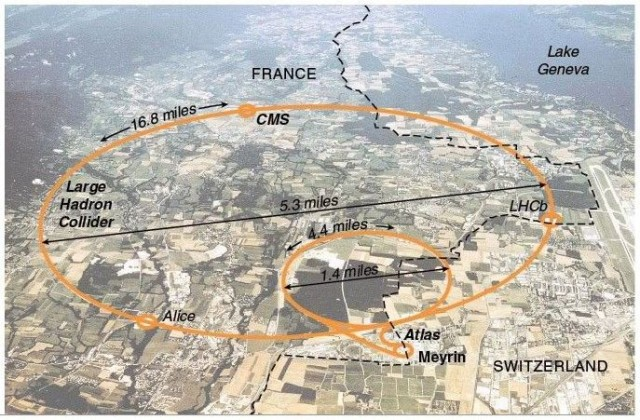
\includegraphics[width=.90\linewidth]{figures/lhc/lhc-5-640x420.jpg}
\caption{The \ac{LHC} main collider ring and pre-accelerator \ac{SPS} overlaid on a map of Switzerland and France, with the four main \ac{LHC} experiments identified.}
\label{fig:lhc_map}
\end{figure}
\end{centering}

%----------------------------------------------------------------------------------------

\section{The Injector Complex}

The goal of the \ac{LHC} is to provide high luminosity proton-proton collisions at 13 \tev. To achieve this, it must be capable of rapidly accelerating large numbers of protons and holding them at a constant energy, and organizing them into bunches which can be focused and collided at precise points and times. To do this, a complex system of pre-accelerators are required, as well as a precisely engineered sytem of magnets withing the \ac{LHC}. The full system of pre-accelerators is shown in \autoref{fig:preacc}.

\begin{centering}
\begin{figure}[!hbt]
\myfloatalign
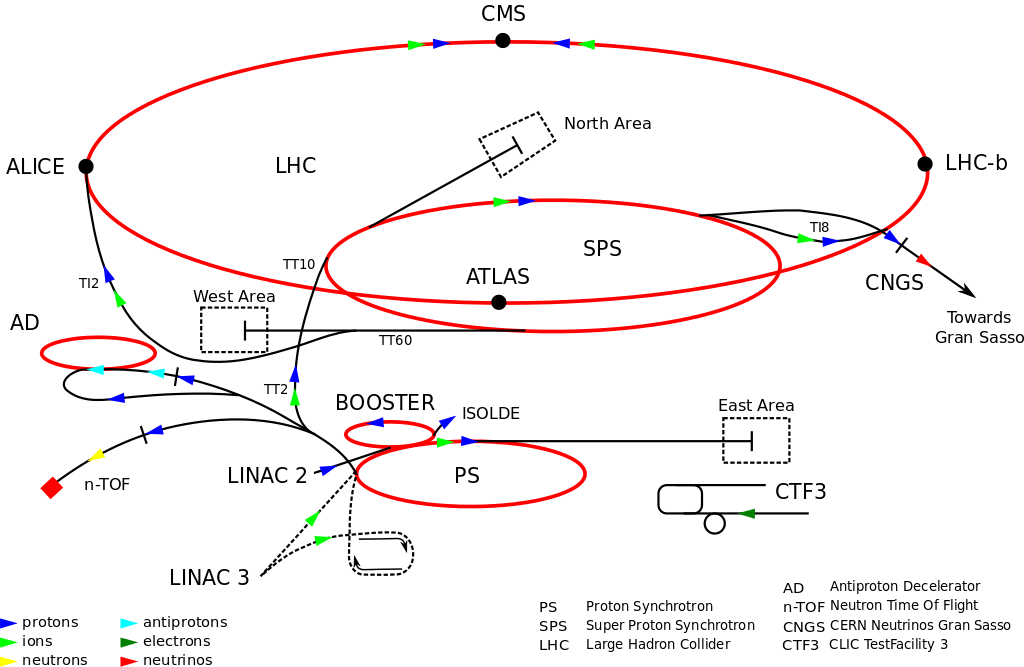
\includegraphics[width=.90\linewidth]{figures/lhc/Cern-accelerator-complex.png}
\caption{The pre-accelerators of the \ac{LHC}}
\label{fig:preacc}
\end{figure}
\end{centering}

The chain begins with when hydrogen gas is stripped of its electrons and injected in short pulses into Linac2, a linear accelerator which uses \ac{RF} cavities, which use alternating positive and negative electric fields to simultaneously push and pull particles forward through the accelerator. Quadropole magnets along the way keep the beam focused. By the end of the accelerator, protons have reached 50 \mev. 

The proton beam is then injected into the \ac{PSB}, the first circular accelerator in the pre-accelerator chain. It increases its magnetic field as the protons increase in speed, ultimately accelerating them to 1.4 \gev. 

At this point the proton moves on to the \ac{PS}, a 600 m long circular accelerator that consists of 277 electromagnets that accelerate the protons up to 25 \gev, and 100 additional dipole magnets to bend the beam. 

The last accelerator before injection into the \ac{LHC} is the \ac{SPS}, a 7 km long ring which is responsible for the discover of the $W$ and $Z$ bosons. The \ac{SPS} accelerates particles up to 450 \gev before they are launched into the \ac{LHC}. It is in this accelerator that the bunch structure 




The \ac{LHC} consists of eight straight sections each connected by an arc, so magnets can alternately accelerate and turn the proton beams. However, because the \ac{LHC} is a proton-proton collider as opposed to a proton-antiproton collider, the two counter-rotating beams must be housed in separate rings and accelerated separately. To achieve this, a twin-bore superconduncting magnet surrounds the two rings and accelerates them both. 










